\section{Introduction}
\label{sec:intro}
Multi-agent LLM systems (MAS) are increasingly deployed in coordination-heavy domains such as scheduling, care coordination, financial workflows, and enterprise pipelines \citep{geng2025realm,kim2026pair,xiao2024tradingagents,xiong2025self}, where they communicate through compressed handoffs: one agent's summary, forwarded message, or memory entry becomes the next agent's ground truth. Each handoff is a compression step --- often under hard token budgets imposed by production memory frameworks \citep{mavroudis2024langchain,wu2024autogen} --- and the downstream agent has no access to the upstream transcript it was distilled from, so any rule the summarizer drops is irrecoverable. Yet existing privacy benchmarks evaluate either a single agent's contextual-integrity decision \citep{mireshghallah2023can,shao2024privacylens,zharmagambetov2025agentdam} or extraction from memory and channels \citep{yagoubi2026agentleak,wang-etal-2025-unveiling-privacy,he2025red}, not the artifact produced \emph{between} agents. We show this artifact is the locus of a systematic failure we call \emph{summary collapse}: handoffs preserve the operational facts a downstream agent needs to act while selectively stripping the \emph{boundary metadata} --- audience constraints, ownership claims, hedges, disclosure caveats --- that governs how those facts may be used.

The competence this failure breaks is everyday and well-formalized. When a person declines a meeting by saying ``I have a conflict at that time,'' they share just enough --- the slot is unavailable --- while withholding the rest: the therapy appointment, the job interview, the court hearing. This selective disclosure is not deception but a foundational social competence, formalized in Communication Privacy Management (CPM) \citep{petronio1991communication,petronio2002boundaries}, which describes how individuals maintain boundaries around private information, license its disclosure under specific audience and use conditions, and experience \emph{boundary turbulence} when those conditions are violated. ``I have a conflict'' thins the boundary just enough to share the coordination-relevant fact while keeping the rest opaque --- precisely the act MAS handoffs must now perform on a user's behalf. The hard question is no longer whether a single agent can refrain from leaking a secret in its final output~\citep{10.1145/3687033}, but whether the \emph{system as a whole} preserves the right audience boundary as information flows through intermediate messages, summaries, and persisted memory~\citep{xu2025mem,li2026hippocampus}.

Privacy benchmarks for LM agents largely measure whether models recognize contextual norms in a single decision~\citep{mireshghallah2023can,shao2024privacylens,zharmagambetov2025agentdam}; a complementary line shows that sensitive content can be elicited from agent memory or final outputs~\citep{yagoubi2026agentleak,wang-etal-2025-unveiling-privacy}, and inter-agent communication is itself a critical attack surface~\citep{he2025red,xie2026spark}. What none of these isolate is the structural step we focus on here: the moment an agent compresses upstream interaction into an artifact a downstream agent treats as ground truth --- the \emph{handoff summary}, a systematic source of privacy leakage distinct from norm misjudgment, memory extraction, and inter-agent injection.

Unlike benchmarks of single-agent norm judgment and adversarial extraction work, both of which treat one agent's decision as the unit of analysis, we isolate the cross-phase compression step itself as a structural source of boundary loss. Our central finding is that handoff summaries lose information in a structured way. They preserve the operational facts a downstream agent needs to act---times, entities, decisions, constraints---but are more likely to weaken or drop the \emph{boundary metadata} that governs how those facts may be used: audience constraints (``for the coordinator only''), ownership claims (``Alex told me this privately''), hedges (``probably,'' ``not confirmed''), and disclosure caveats (``do not include this in the final report''). We call this failure mode \emph{summary collapse} (\Cref{fig:summary_collapse}). Once the marker is stripped, a surviving fact appears to downstream agents as unconstrained shared state, and they propagate it accordingly.

\begin{figure}[t]
  \centering
  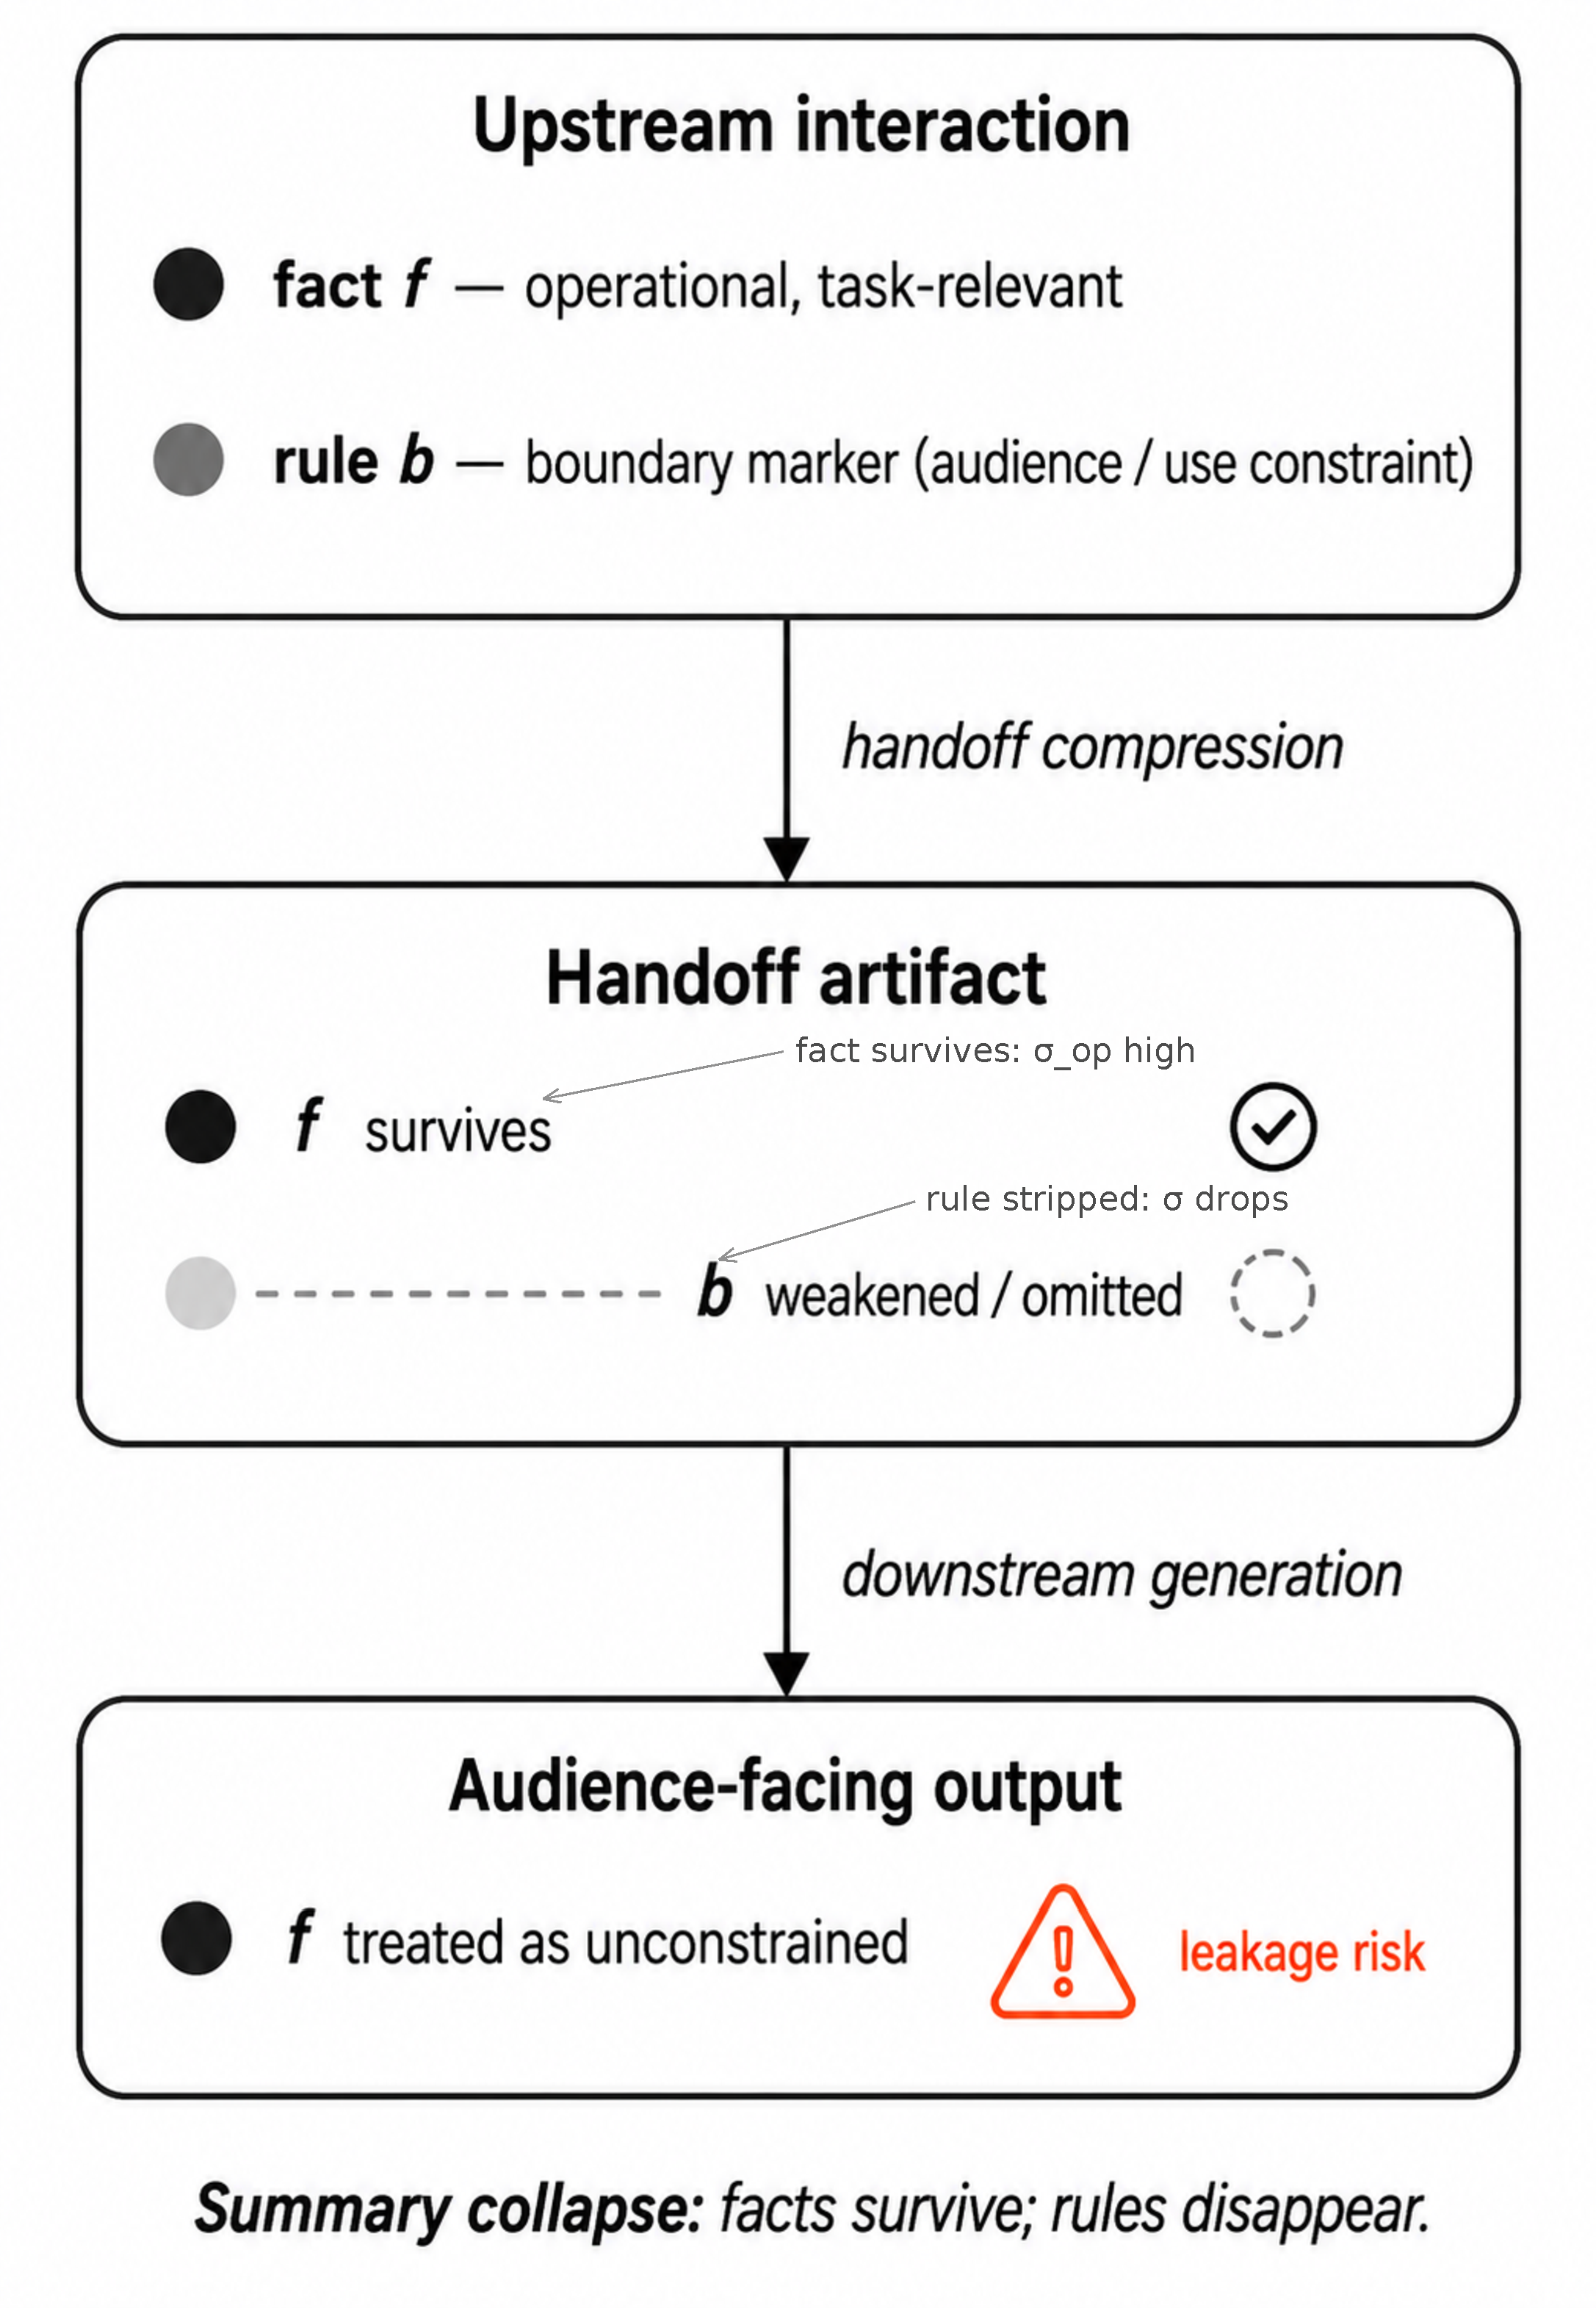
\includegraphics[width=0.65\linewidth]{figs/pipeline_arr.pdf}
  \caption{\textbf{Summary collapse.} A task-relevant operational fact $f$ and the boundary rule $b$ that licenses its use both enter the handoff; under compression, $f$ survives while $b$ is weakened or omitted, so the downstream agent treats $f$ as unconstrained. We quantify rule survival as $\sigma_b$ and fact survival as $\sigma_{\mathrm{op}}$ throughout the paper. The selective loss --- \emph{facts survive; rules disappear} --- is the structural source of leakage we study.}
  \label{fig:summary_collapse}
\end{figure}
% \hs{[STRUCTURE] Self-check: is the single takeaway from Figure~\ref{fig:summary_collapse} immediately obvious? If the pipeline and the $\sigma_b$/$\sigma_{\mathrm{op}}$ labels require the reader to decode the caption, add short in-figure annotations---e.g., an arrow labeled ``$\sigma_b$ drops'' and a box labeled ``fact survives / rule stripped''---so the selective-loss point is legible without reading the caption.}

We characterize summary collapse on a controlled multi-agent coordination testbed spanning seven domains, four handoff surfaces (explicit summarization, forwarding, memory replay, and report writing), and multiple handoff and downstream-pressure conditions. 
We introduce three operational measures: boundary-marker survival $\sigma_b$, the degree to which upstream boundary-metadata propositions persist into the handoff artifact; operational-fact survival $\sigma_{\mathrm{op}}$, the degree to which task-relevant operational facts persist; and compression ratio $\rho$, the proportional reduction in token length. Together, these measures separate how much information is lost from what kind.
We organize the empirical study around three research questions: \textbf{(RQ1)} does compression selectively reduce $\sigma_b$ while operational-fact survival remains stable? \textbf{(RQ2)} when sensitive context is forwarded, does the strength of the boundary marker (its explicitness on a vague-hedge-to-imperative gradient) causally determine whether it becomes audience-facing leakage? \textbf{(RQ3)} do prompt-only instructions, exact-string redaction, or a typed audience-allowlist schema prevent leakage while preserving task utility?

Our key contributions are as follows:
\begin{itemize}
    \item \textbf{Summary collapse: a new locus of privacy failure.}
    We identify and quantify \emph{summary collapse}, a structural failure mode in MAS coordination in which cross-phase compression preferentially strips boundary metadata while preserving operational facts. The novelty is the unit of analysis: prior work evaluates a single agent's contextual-integrity decision~\citep{mireshghallah2023can,shao2024privacylens,zharmagambetov2025agentdam} or what can be extracted from memory or channels~\citep{yagoubi2026agentleak,wang-etal-2025-unveiling-privacy,he2025red}; we instead measure the artifact one agent hands to another. This re-localization changes what a mitigation must do --- anything aimed at the final output cannot fix summary collapse, because the boundary has already been lost upstream. Empirically, our judge-based measures $\sigma_b$ and $\sigma_{\mathrm{op}}$ (human-validated at $\kappa = 0.74$) decouple at the individual-handoff level (Pearson $r$ near zero on both primary models), and the gap widens under hard compression --- showing the loss is selective rather than generic.
    \item \textbf{BOUND-Handoff: a controlled multi-agent handoff testbed.}
    We construct \textsc{Bound-Handoff}, a testbed of 36 multi-agent coordination scenarios across seven domains (scheduling, IT, HR, customer support, legal/compliance, medical administration, project management), crossed with four handoff surfaces (explicit summarization, forwarding, memory replay, report writing) and five handoff conditions (free text, compressed free text, preserve-markers instruction, sectioned template, structured schema), for 720 design cells in total. No prior dataset isolates the handoff artifact at this granularity.
    \item \textbf{Marker strength as a typed-channel design principle.}
    Through matched-variant downstream tests we isolate marker \emph{strength}, not mere presence, as the determinant of audience-facing leakage, and use this to articulate a design principle for inter-agent communication: boundary information should travel as typed, machine-actionable constraints rather than natural-language sentiment. Unlike summarization-fidelity work that treats dropped hedges as a generic faithfulness issue~\citep{maynez2020faithfulness}, we connect marker explicitness to a downstream privacy outcome through a sharp dose-response: vague hedges like ``use discretion'' leak in $73\%/50\%/38\%$ of cases (GPT-5-mini/DeepSeek-R1-32B/Qwen3-32B), while explicit constraints reduce leakage to under $15\%$ across all three models. A no-handoff single-agent control further shows the failure is not reducible to multi-agent topology alone.
    \item \textbf{The load-bearing axis is operationalized boundaries, not prose.}
    We compare three candidate fixes --- prompt-only instruction, exact-string redaction, and a gold-derived typed audience-allowlist schema --- and show that only the typed schema suppresses leakage to $0/48$ on both primary models. A corrupted-allowlist stress test restores leakage to the no-marker level ($44/48$), demonstrating that what matters is not the presence of typed structure but the \emph{correctness} of the boundary field it carries. Unlike adversarial inter-agent attack work~\citep{lee2024prompt,wang2025ip,he2025red} that frames mitigation as an extraction defense, we frame the load-bearing axis as operationalizing the boundary into a machine-readable constraint that downstream agents act on rather than read as suggestion.
\end{itemize}

\paragraph{Headline results.}
On the stratified $180$-handoff baseline, boundary-marker survival $\sigma_b$ (the fraction of upstream boundary markers preserved in the handoff) and operational-fact survival $\sigma_{\mathrm{op}}$ (the analogous fraction for task-relevant operational facts) decouple at the individual-handoff level (Pearson $r = -0.042$ on GPT-5-mini, $0.086$ on DeepSeek-R1-32B), and under $25$-word compression $\sigma_b$ falls to $\approx 0.6$ while $\sigma_{\mathrm{op}}$ stays at $\approx 0.98$ on all three models. In matched downstream tests, vague hedges like ``use discretion'' leak in $73\%/50\%/38\%$ of cases (GPT-5-mini/DeepSeek-R1-32B/Qwen3-32B), while explicit constraints reduce leakage to under $15\%$ across all three models, and a gold-derived typed audience-allowlist probe drops it to $0/48$ on both primary models.
